\documentclass{beamer}
\mode<beamer>{%
\usetheme[hideothersubsections,
right,width=22mm]{Goettingen}
}
\usepackage[spanish]{babel} %Definir idioma español
\usepackage[utf8]{inputenc} %Codificacion utf-8
\title{Análisis sintáctico de la lógica de primer orden}
\author{Emmanuel Peto Gutiérrez}
\institute{IIMAS \\ UNAM}
\begin{document}

\begin{frame}<handout:0>
\titlepage
\end{frame}

\section{Descripción del problema}

% 1
\begin{frame}
\frametitle{Razonamiento automatizado}

El razonamiento automatizado es el área de las ciencias de la computación concentrada en aplicar el razonamiento de forma lógica a un sistema.

Dados un conjunto de hipótesis y una meta, un sistema de razonamiento automatizado debería hacer inferencias lógicas para llegar a la meta automáticamente.

\pause

Si hago un programa que haga inferencia, el primer problema a resolver es el de darle la entrada al programa. ¿Cuál es el formato que entiende mi programa?

\end{frame}

% 2
\begin{frame}
\frametitle{Gramática en lógica de primer orden}

Lenguajes como Haskell nos permiten definir gramáticas.

Lo que entendemos nosotros:

$t$ ::= $x | f [t]$

$at$ ::= $\top | \bot | P [t] | t=t$

$\star$ ::= $\rightarrow | \leftrightarrow | \land | \lor$

$Q$ ::= $\forall | \exists$

$f$ ::= $at | f \star f | Q x f$

\pause

Lo que entiende Haskell:

\texttt{data Term = Var String | Fun String [Term]}

\texttt{data Form  = Top | Bot | Pred String [Term] | Eq Term Term | Neg Form | Or Form Form | And Form Form | Impl Form Form | Syss Form Form | Forall String Form | Exists String Form}

\end{frame}

% 3
\begin{frame}
\frametitle{Parser}

Problema: construir un programa que lea cadenas de texto (sintaxis concreta) y lo transforme a una expresión que sea entendible por Haskell (sintaxis abstracta).

\end{frame}

\section{Análisis léxico y sintáctico}

% 4
\begin{frame}
Traducir de sintaxis concreta a sintaxis abstracta es un tema bien conocido porque es de central importancia en lenguajes de programación. Es convencional separar la transformación en dos pasos:

\pause

\begin{itemize}
\item \textbf{Análisis léxico:} descomponer el texto de entrada en ``tokens''.

\pause

\item \textbf{Análisis sintáctico:} convertir la sucesión de tokens en un árbol de sintaxis abstracta.
\end{itemize}

\end{frame}

\section{Análisis de términos}

% 5
\begin{frame}
\frametitle{Términos}

El primer paso es construir un parser de términos.

Contrato:
\begin{itemize}
\item Si al término lo precede una `c', es constante.
\item Si lo precede una `v', es variable.
\item Si lo precede una `f', es función.
\end{itemize}

La función que realiza el análisis sintáctico de un término se llama \texttt{parseTerm}.

Ejemplo:

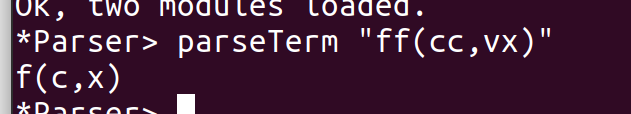
\includegraphics[scale=0.3]{parseTerm.png}

\end{frame}

\section{Análisis de fórmulas}

% 6
\begin{frame}
\frametitle{Tokens}

El primer paso para analizar una fórmula es separar el texto en tokens, donde un token será un par (\texttt{tipo}, \texttt{token}). Es decir, cada token estará unido con su tipo.

Los diferentes tipos de tokens son: cuantificador, paréntesis izquierdo, paréntesis derecho, predicado, conector.

Ejemplo:

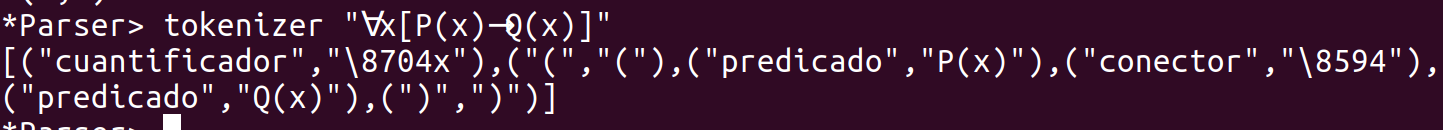
\includegraphics[scale=0.2]{tokenizer.png}

\end{frame}

% 7
\begin{frame}
\frametitle{Notación postfija}

El segundo paso es transformar los tokens de notación infija a postfija. En este paso se eliminarán los paréntesis.

Ejemplo:

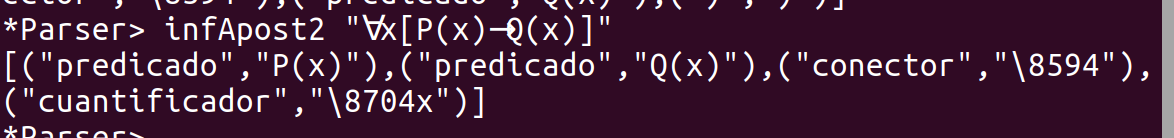
\includegraphics[scale=0.2]{postfija.png}

\end{frame}

% 8
\begin{frame}
\frametitle{Sintaxis abstracta}

En el último paso, se toma una expresión de tokens en notación postfija y se transforma a una fórmula de Haskell (definida con \texttt{data Form}).

Ejemplo:

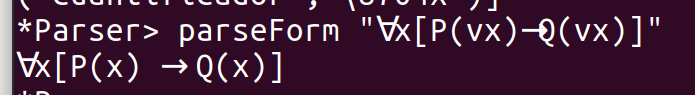
\includegraphics[scale=0.3]{parseForm.png}

\end{frame}

\section{Locally nameless representation}

% 9
\begin{frame}
\frametitle{Alfa-equivalencias}

Uno de los problemas que surgen en la representación con nombres es que dos fórmulas pueden ser distintas aunque el significado sea el mismo. Cuando esto ocurre, se dice que son \textit{$\alpha$-equivalentes}.

Ejemplo, las siguientes fórmulas son $\alpha$-equivalentes: $\forall x P(x)$ y $\forall y P(y)$.

Si le preguntamos a Haskell si las fórmulas son iguales nos va a decir que no (imprime False).

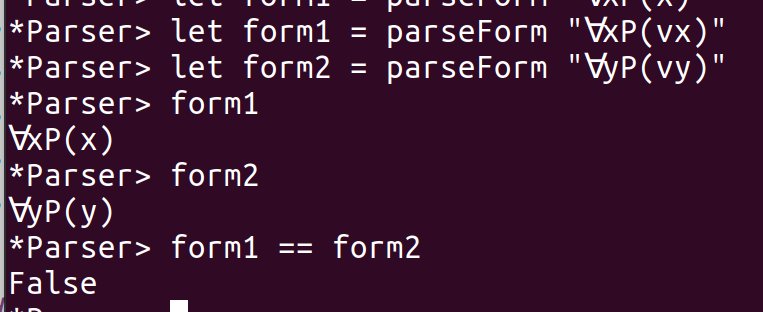
\includegraphics[scale=0.25]{alfa.png}

\end{frame}

% 10
\begin{frame}
\frametitle{Representación local sin nombres}

Se pueden representar las fórmulas y términos con una gramática diferente, la cual quita los nombres de las variables ligadas y pone números. A esos números se les conoce como índices de de Bruijn.

Una variable con índice $i$ apunta al $(i+1)$-ésimo cuantificador que lo encierra. Además, la gramática hace una diferencia explícita entre las variables ligadas (\texttt{Bvar}) y las libres (\texttt{Fvar}). La nueva gramática es la siguiente, donde $t$ son los términos y $form$ las fórmulas.

\begin{itemize}
\item $t$ ::= Bvar $i$ $|$ Fvar $name$ $|$ f $name$ [t]
\item $form ::=  \forall form | \exists form$ ...
\end{itemize}

Nota: los puntos suspensivos en $form$ significan que el resto de la gramática se queda igual.

\end{frame}

% 11
\begin{frame}
\frametitle{Transformación de fórmulas}

Se realizó una función que transforma fórmulas \textit{crudas} a su equivalente en representación local sin nombres.

Si se tienen dos fórmulas $\alpha$-equivalentes tal que no tienen variables libres, entonces se verán exactamente igual en su representación sin nombres.

Ejemplo:

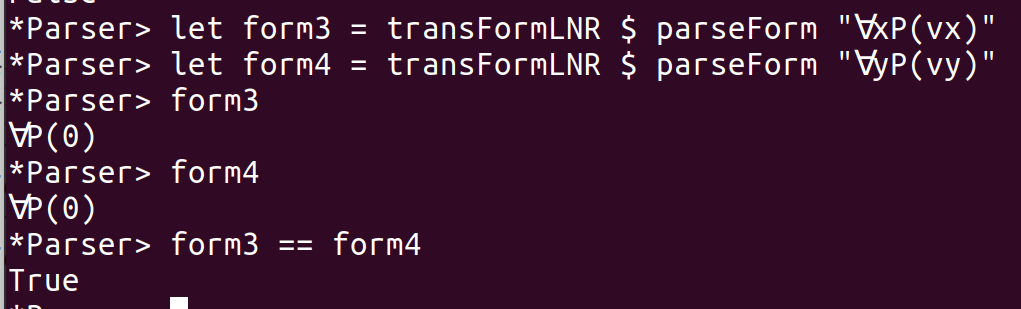
\includegraphics[scale=0.25]{nameless.png}

\end{frame}

% 12
\begin{frame}

\centering
{\Huge FIN}

\end{frame}

\end{document}

